\section{Arbeitsgrundlagen}

Die Polarisation bei Wellen betrifft die Schwingungsrichtung der Wellenerregung.
Bei  Longitudinalwellen  besteht  diesbez\"uglich  keine Freiheit,  weshalb  der
Begriff nur  f\"ur  Transversalwellen sinnvoll ist. Von hervorragender Bedeutung
ist die Polarisation bei elektromagnetischen Wellen, insbesondere beim Licht, wo
sie  mit  zahlreichen wichtigen Ph\"anomenen verkn\"upft ist. Wir  beschr\"anken
uns im folgenden auf diese Wellenart.

Eine  fortschreitende  elektromagnetische   Welle   erzeugt   lokal  --  in  der
Normalebene zur Laufrichtung  --  ein  variables  elektrisches  Feld, welches in
einem  Medium  Elektronen in  Bewegung  setzt.  Diese  bewegten  Ladungstr\"ager
k\"onnen  wir  dann   nach   dem   Huygens'schen  Prinzip  als  Elementarquellen
betrachten, von denen eine ihrer Bewegung entsprechende Welle ausgeht. Wegen des
Satzes  von  Fourier  gen\"ugt es, harmonische Wellen zu betrachten.  F\"ur  die
untenstehenden   Ausf\"uhrungen  gelten  folgende  Konventionen/Voraussetzungen:

\begin{itemize}
    \item wir beschr\"anken uns auf harmonische, quasimonochromatische, ebene Wellen
    in linearen Medien
    \item die Lichtausbreitung erfolgt standardm\"assig in z-Richtung
    \item  es  wird  jeweils  nur  das elektrische Feld erw\"ahnt/gezeichnet, da die
    magnetische Feldst\"arke dadurch automatisch festgelegt ist
    \item  der  Unterschied  von  Wellennormalen  (Richtung  des  Wellenvektors) und
    Energieausbreitungsrichtung (Richtung des Poyntingvektors) in anisotropen Medien
    wird vernachl\"assigt.
\end{itemize}

In Isotropen Medien kann der Feldst\"arke als Summe von zwei Teilvektoren geschrieben werden.

\begin{equation}
    \vec{E}(z,t) = \begin{pmatrix}
        \hat{E}_x\cdot\cos(k \cdot z - \omega t - \delta_x) \\
        \hat{E}_y\cdot\cos(k \cdot z - \omega t - \delta_y) \\
    \end{pmatrix}
    \label{eq:welle}
\end{equation}

Das  Amplitudenverh\"altnis  $E_x/E_y$  sowie  die  relative  Phase $\delta_x  -
\delta_y$  bestimmt   den  Typus  der  Polarisation  respektive  der  Typus  der
Polarisation bestimmt die Wahl des Koordinatensystems.


\subsection{Lineare Polarisation}

Lineare  Polarisation  liegt  vor,  wenn die lokale Schwingung des  elektrischen
Feldes   bzw.   die    Bewegung   der   Elementarzentren   linear   ist.   Diese
Schwingungsrichtung  ist identisch mit  der  Polaristationsrichtung  der  Welle.

In anderen Worten, die Welle liegt in der Ebene bei einem konstanten Winkel, und
die  Phasenverschiebung $\delta$ der vorhin beschriebenen Teilvektoren ist Null.
Die Figur \ref{fig:linear_pol} zeigt, wie ein nicht  polarisiertes  Licht linear
polarisiert wird.

\begin{figure}[H]
    \centering
    \begin{subfigure}{.45\linewidth}
        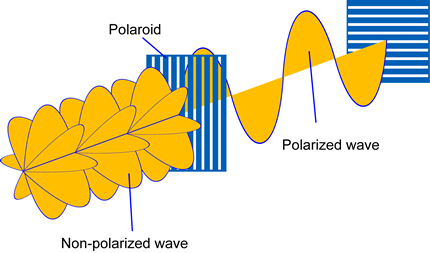
\includegraphics[width=.95\linewidth]{images/polarisation.png}
        \caption{Nicht-polarisiertes Licht wird durch ein Polarisator linear polarisiert.}
        \label{fig:linear_pol}
    \end{subfigure}
    \begin{subfigure}{.45\linewidth}
        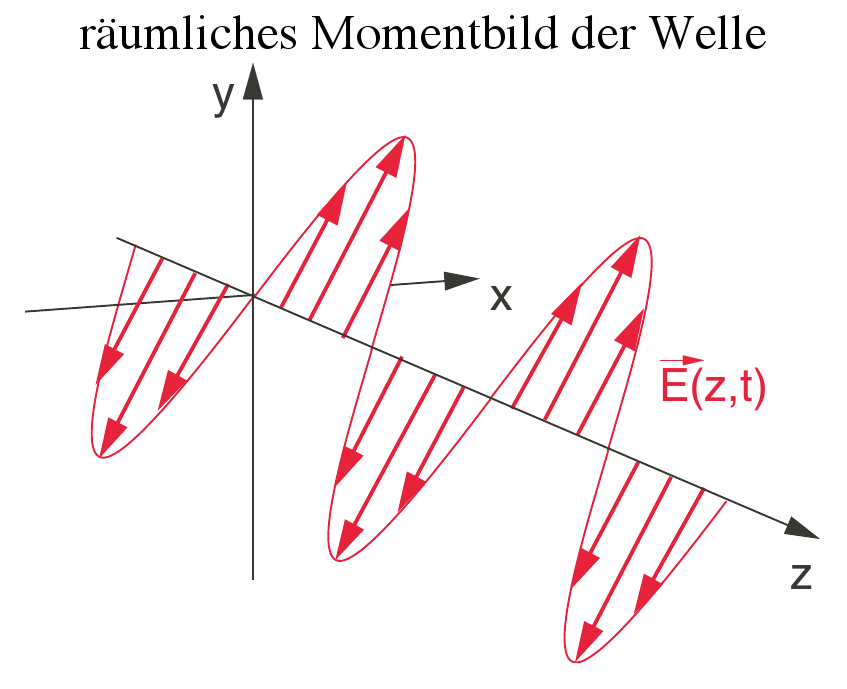
\includegraphics[width=.99\linewidth]{images/polarisation-linear.png}
        \caption{R\"aumliches Momentanbild einer linear polarisierten Welle}
    \end{subfigure}
\end{figure}

Aus der Formel \ref{eq:welle} mit $\delta=0$ folgt:

\begin{equation}
    R = \vec{E}(z,t) = \begin{pmatrix} \hat{E}_x \\ \hat{E}_y \end{pmatrix} = \cos(k \cdot z - \omega t)
\end{equation}

Die Zerlegung (Wahl von x- und y-Achse) in  zwei Teilwellen ist nicht eindeutig,
sie  kann  der  physikalischen  Situation angepasst werden. Die  Umrechnung  der
Teilamplituden  vom  einen  Koordinatensystem   ins   andere   erfolgt  mit  der
Rotationsmatrix:

\begin{equation}
    \begin{pmatrix}
        \cos\varphi  & \sin\varphi \\
        -\sin\varphi & \cos\varphi \\
    \end{pmatrix}
\end{equation}

Wenn eine linear polarisierte Welle durch einen Polarisator tritt, dann wird die
x-Teilwelle geblockt und die  y-Teilwelle  durchgelassen.  Dieses Verhalten kann
mit der Matrix

\begin{equation}
    \begin{pmatrix}
        1 & 0 \\ 0 & 0 \\
    \end{pmatrix}
\end{equation}

beschrieben   werden.   Dabei   ist  zu  verstehen,  dass  ``x''  und  ``y''  im
Koordinatensystem vom Polarisator ist.  Die  Teilwellenkomponenten m\"ussen also
zuerst in das Koordinatensystem vom Polarisator transformiert werden,  und  dann
wieder zur\"ucktransformiert werden.

\begin{equation}
    \vec{E}_{out} = \begin{pmatrix}
        \cos\varphi & -\sin\varphi \\
        \sin\varphi &  \cos\varphi \\
    \end{pmatrix}\begin{pmatrix}
        1 & 0 \\ 0 & 0 \\
    \end{pmatrix}\begin{pmatrix}
        \cos\varphi  & \sin\varphi \\
        -\sin\varphi & \cos\varphi \\
    \end{pmatrix} \cdot\vec{E}_{in}
    \label{eq:polarisator}
\end{equation}

Durch   Vektorzerlegung  der  Formel   \ref{eq:polarisator}   kann   f\"ur   ein
Polarisator/Analysator-Paar  eine  einfache  Formel  hergeleitet werden, der die
Transmission beschreibt:

\begin{equation}
    I_{out} = I_0 \cdot \cos^2(\varphi)
    \label{eq:pol_paar}
\end{equation}


\subsection{Elliptische und Zirkulare Polarisation}

Ist  die  relative  Phase  zwischen  den zwei  linear  polarisierten  Teilwellen
ungleich  Null  (oder  $\pi$),  verteilen wir den Phasenunterschied $\delta$ auf
beide Teilwellen und schreiben.

\begin{equation}
    \vec{E}(z,t) = \begin{pmatrix}
        \hat{E}_x\cdot\cos(k \cdot z - \omega t - \delta/2) \\
        \hat{E}_y\cdot\cos(k \cdot z - \omega t + \delta/2) \\
    \end{pmatrix}
    \label{eq:ellip}
\end{equation}

Die Funktion $\vec{E}(z,t)$  beschreibt nun eine Ellipse -- oder im Spezialfall,
wenn  $\hat{E}_x=\hat{E}_y$  und $\delta=\pm\pi/2$,  ein  Kreis.  Die  Abbildung
\ref{fig:zirkular_pol} zeigt eine grafische Darstellung.

\begin{figure}[H]
    \centering
    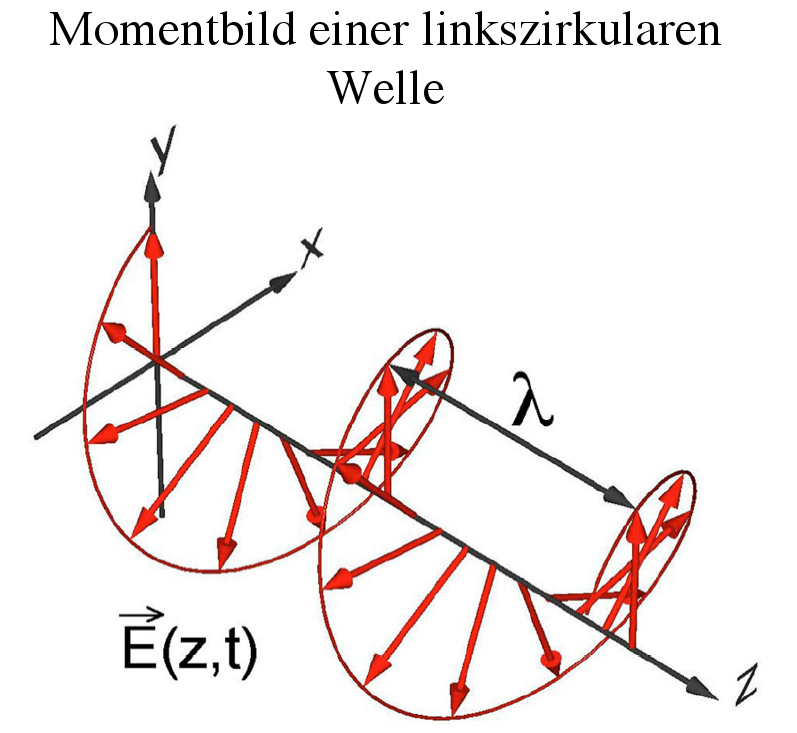
\includegraphics[width=.5\linewidth]{images/polarisation-zirkular.png}
    \caption{R\"aumliches Momentanbild einer zirkular polarisierten Welle}
    \label{fig:zirkular_pol}
\end{figure}

Die elliptische Polarisation kommt zustande, wenn eine linear polarisierte Welle
durch ein anisotropes Medium tritt. Beispiele f\"ur solche Medien sind Kristalle
(z.B.  Quarz)  oder  Kunststoffe  mit  ausgerichteten   Molek\"ulen.   Weil  der
Brechungsindex $n$ in diesen Medien richtungs- und polarisationsabh\"angig  ist,
werden die zerlegten Teilwellen einer linear polarisierten Welle unterschiedlich
verz\"ogert  -- d.h. es entsteht eine Phasenverschiebung $\delta$.

Das Verhalten von Wellen  in anisotropen Medien wird beschrieben mit der Formel:

\begin{equation}
    \vec{E}(z,t) = \begin{pmatrix}
        \hat{E}_x\cdot\cos(k_x \cdot z) - \omega t - \delta/2 \\
        \hat{E}_y\cdot\cos(k_y \cdot z) - \omega t - \delta/2 \\
    \end{pmatrix}
\end{equation}

Wobei   $k_x   =   n_x   \cdot   \frac{\omega}{c_0}$   und  $k_y  =  n_y   \cdot
\frac{\omega}{c_0}$.   $n_x$   ist   der  Brechungsindex  f\"ur  die  x-Richtung
polarisierte Teilwelle,  $n_y$  ist  der  Brechungsindex  f\"ur  die  y-Richtung
polarisierte Teilwelle.

Eine  sogenannte  Wellenplatte  verz\"ogert  die eine  Teilwelle  um  die  Phase
$\epsilon$ relativ  zur  anderen.  Die  Polarisationsrichtung  mit dem kleineren
Brechungsindex  heisst  die  schnelle  Achse  der  Wellenplatte.  Verteilen  wir
gem\"ass Konvention die Phase auf beide Teilwellen, so erhalten wird die Matrix:

\begin{equation}
    M = \begin{pmatrix}
        e^{-i\epsilon/2} & 0 \\
        0 & e^{ i\epsilon/2} \\
    \end{pmatrix}
\end{equation}

Eine Lambdaviertelplatte wird folglich repr\"asentiert durch:

\begin{equation}
    M = \begin{pmatrix}
        e^{-i\pi/4} & 0 \\
        0 & e^{ i\pi/4} \\
    \end{pmatrix}
\end{equation}

Die Strahlungsintensit\"at kann berechnet werden, indem die x- und y-Komponenten quadriert und addiert werden.

\begin{equation}
    I = I_0 \cdot \left(E_xE^*_x + E_yE^*_y\right)
    \label{eq:intensitaet}
\end{equation}

$E_x^*$ und $E_y^*$ sind komplex konjugiert.
